%! TEX program = lualatex
%! TEX root = thesis.tex

% DocumentMetadata is required for an accessible PDF
\DocumentMetadata{
    lang=en,
    pdfstandard=ua-2,
    tagging=on,
    tagging-setup={
        math/setup={mathml-AF,mathml-SE},
        extra-modules={verbatim-mo},
    }
}
\documentclass{uofithesis}
% \documentclass[thesis]{uofithesis} % for a thesis

% fontsetup can slow down compilation, so you may wish to omit it when writing
% \usepackage{fontsetup}

% If using math unicode-math is required for math accessibility.
% If not using math, remove this package.
\usepackage{unicode-math}

% Remove any graphics packages you are not using.
% Graphics packages can be used as long as alt-text is provided.
% For tikz alt text can be added with:
%   \begin{tikzpicture}[alt={Alt text...}]
% For images:
%  \includegraphics[alt={Alt text...}]{image.png}
\usepackage{graphicx}
\usepackage{tikz}
% uofithesis sets accessible colors for use in charts, but you can also define
% your own if needed
\usepackage{pgfplots}

\usepackage{csquotes}

% Bibliography for references
% biber must be set as the backend, style can be changed as needed
\usepackage[hidelinks,pdfusetitle]{hyperref}
\usepackage[backend=biber,style=ieee]{biblatex}
\usepackage[bottom]{footmisc}

% At time of writing, chemistry packages are not compatible with accessibility
% tagging, but there are no alternatives.
% \usepackage[version=4]{mhchem}
% \usepackage{chemfig}
% \pgfplotsset{compat=1.18}

\addbibresource{./references.bib}

% Raggedright is recommended for accessibility
\raggedright
\setlength{\parindent}{1.5em}

\title{Microwave Spectroscopy in Planar Josephson Junctions}
\author{Randy Owen}
\department{Physics}

% You can set a specific earned degree instead of Master/Doctor of Science/Philosophy
%\earneddegree{Doctor of Education}

% Add a concentration if applicable
%\concentration{Coffee Studies}
% Add a minor if applicable
%\minor{Global Studies}

\degreeyear{2026}

% You can set a custom text for the committee section, otherwise it will default
% to "Doctoral Committee:" or "Master's Committee:" based on the degree level
%\committeetitle{Advisers:}

\committee{
\item Associate Professor Bob Barnard, Chair
\item Assistant Professor Charlie Clarke
\item Professor Dan Drower
\item Professor Eve Earlsfield
}
\includeonly{Chapter/Introduction}
\begin{document}


% Uncomment the copyrightpage macro to include an automatic copyright page
% before the title
%\copyrightpage
\maketitle

\abstract{
    This is the abstract of the thesis. It should be a concise summary of the
    research, including the main findings and conclusions. The abstract should
    be no more than 350 words in length.
}

\acknowledgements{
    This page is optional. The text should be in either 10- or 12-point font
    and the line spacing should be either 1.5 or double-spaced.

    If you do not want to include an acknowledgment, delete the text of the
    acknowledgment and the \texttt{\textbackslash acknowledgements} command
    from your \texttt{.tex} file.
}

% dedication uses begin and end syntax because it opens a center environment
% which needs to be closed
\begin{dedication}
    A dedication is optional.
\end{dedication}

\tableofcontents


%!TEX root = ../thesis.tex
% \chapter{Introduction}
\section{Are ABS cool?}
ABS are cool.
%!TEX root = ../thesis.tex
\section{Coffee Berries}

A coffee bean is a seed from the Coffea plant and the source for coffee. This
fruit is often referred to as a coffee cherry, but unlike the cherry, which
usually contains a single pit, it is a berry most commonly found having two
seeds with their flat sides together.

\tagstructbegin{tag=Part}
\begin{figure}[H]
    \centering
    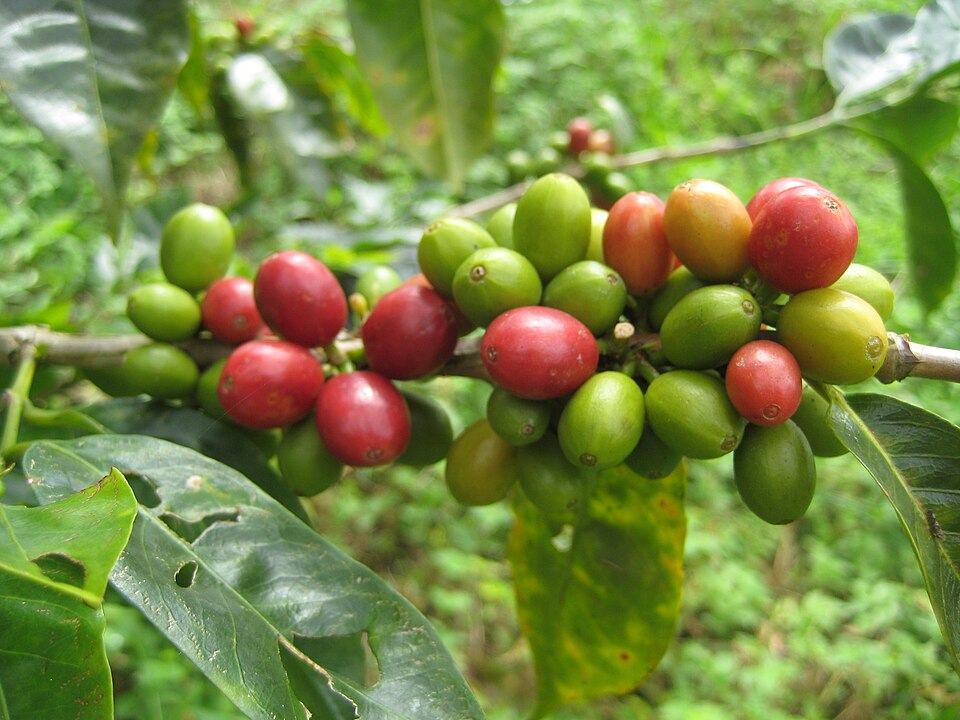
\includegraphics[width=0.6\textwidth,alt={Multiple red and green coffee
    berries clustered together on coffee tree branches}]{
        Clumps_of_coffee_berries_growing_on_a_tree_by_Brian_Smith.jpg
    }
    \caption{Clumps of coffee berries growing on a tree (Photo by Brian Smith)}
    \label{fig:coffee_berries}
\end{figure}
\tagstructend

\subsection{Characteristics of Coffee Berries}

The two most economically important varieties of coffee plants are the arabica
and the robusta; approximately 60\% of the coffee produced worldwide is arabica
and some 40\% is robusta.

\tagstructbegin{tag=Part}
\begin{table}[H]
    \centering
    \caption{Common Coffee Species Comparison}
    \medskip
    \label{tab:coffee_species}
    \renewcommand{\arraystretch}{1.5}
    \tagpdfsetup{table/header-columns={1},table/header-rows={1}}
    \begin{tabular}{|>{\bfseries}l|l|l|}
        \hline
        Species & \textbf{Flavor Profile} & \textbf{Global Production} \\
        \hline
        Arabica & Smooth, complex, with fruit notes & 60\% \\
        \hline
        Robusta & Strong, bitter, earthy & 40\% \\
        \hline
    \end{tabular}
\end{table}
\tagstructend
\pagebreak

The following table summarizes key information about coffee berries:

\tagstructbegin{tag=Part}
\begin{table}[H]
    \centering
    \caption{Key Characteristics of Coffee Berries}
    \medskip
    \label{tab:coffee_characteristics}
    \renewcommand{\arraystretch}{1.5}
    \tagpdfsetup{table/header-columns={1}}
    \begin{tabular}{|>{\bfseries}p{2in}|p{4in}|}
        \hline
        Color at Ripeness & Bright red, yellow or pink depending on variety \\
        \hline
        Size & Approximately 15 mm in diameter \\
        \hline
        Weight & 300--330 mg dry \\
        \hline
        Seeds per Berry & Typically 2 seeds; 10--15\% are peaberries (single seed) \\
        \hline
        Time to Maturity & 6--11 months depending on variety and growing conditions \\
        \hline
        Caffeine Content & 1.0--2.5\% by dry weight \\
        \hline
        Growing Conditions & Altitudes of 600--2,200 meters; temperatures of 15--24°C \\
        \hline
        Shelf Life (Fruit) & 2--3 weeks if left on tree after ripening \\
        \hline
    \end{tabular}
\end{table}
\tagstructend
%!TEX root = ../thesis.tex

\section{Coffee Charts}

Data visualization is an important aspect of understanding coffee consumption
patterns and production statistics. The following chart displays typical daily
coffee consumption at different times.

\tagstructbegin{tag=Part}
\begin{figure}[H]
    \begin{tikzpicture}[alt={Bar chart showing a marked increase in coffee
        consumption during deposit week with a steep decline after deposit}]
        \begin{axis}[
                width=0.9\textwidth,
                height=3in,
                ybar,
                cycle list name=StrictAA,
                every axis plot/.append style={fill, draw=black},
                nodes near coords style={text=black, font=\small},
                enlargelimits=0.15,
                ylabel={Avg. Cups per Day},
                symbolic x coords={Weekday, Weekend, Deposit Week, Post-Deposit},
                xtick=data,
                nodes near coords,
                nodes near coords align={vertical},
                bar width=20pt
            ]
            \addplot+ coordinates {(Weekday,2.1) (Weekend,1.4) (Deposit Week,4.6) (Post-Deposit,0.3)};
        \end{axis}
    \end{tikzpicture}
    \caption{Average Daily Coffee Consumption By Period}
    \medskip
    \label{fig:coffee_consumption_chart}
\end{figure}
\tagstructend
\bigskip

The following line chart illustrates the trend of coffee consumption throughout
a week. There is a noticeable increase in consumption during the middle of the
week, peaking on Thursday and Friday, followed by a decline over the weekend.

\tagstructbegin{tag=Part}
\begin{figure}[H]
    \centering
    \begin{tikzpicture}[alt={Line chart showing the trend of coffee consumption
        throughout the week, with a peak on Thursday and Friday}]
        \begin{axis}[
                width=0.9\textwidth,
                height=5cm,
                xlabel={Day of Week},
                ylabel={Cups Consumed},
                legend style={at={(0.5,-0.15)},
                anchor=north,legend columns=-1},
                grid=major,
                xtick={1,2,3,4,5,6,7},
                xticklabels={Mon, Tue, Wed, Thu, Fri, Sat, Sun},
            ]
            \addplot[mark=*] coordinates {(1,2.4) (2,2.6) (3,2.8) (4,3.2) (5,3.5) (6,1.8) (7,1.2)};
            \legend{Daily Intake}
        \end{axis}
    \end{tikzpicture}
    \caption{Coffee Consumption Trend Throughout the Week}
    \medskip
    \label{fig:coffee_trend_chart}
\end{figure}
\tagstructend




% \printbibliography[heading=bibintoc,title={References}]

\appendices{
    \input{Chapters/appendix_1}

}
\end{document}
